%! TeX root = ../charles/en/thesis.tex
\chapter{Related Work}
\label{chap:rel}

This chapter looks at previous work on probing \acrlongpl{vlm},
and techniques for improving reasoning in various directions in \acrlong{vlm}s. We use
and extend the approaches explored to try and improve the temporal reasoning
abilities of \acrlongpl{vidlm}.

%\section{Video Language Models}
%\label{sec:vidlmb}
%
%CLIP-based \citep{radford2021clip} with no video data, 
%Contrastive with video data, Merlot Reserve~\cite{zellers2022mreserve}, VideoCLIP~\cite{xu2021videoclip}, \cite{luo2022clip4clip}
%Masked VLM: VideoBERT \citep{sun2019videobert}, VLM \citep{xu2021vlm}
%Separate frozen image/video approaches with finetuning/adapters: Flamingo \citep{alayrac2022flamingo}
%Separate frozen image/video approaches with prompt engineering: \citep{wang2022vidil, zeng2023socratic}


\section{Contrastive Training in \acrshortpl{vlm}}
\label{sec:contrastive}

Some previous studies have looked at the effect of contrastive pre-training in
vision and language models, and introduce the idea of post-pretraining VLMs
with hard negatives~\citep{yuksekgonul2023when, momeni2023verbs,
bagad2023testoftime}. Post-pretraining is a continuation of self-supervised
pre-training on a smaller dataset with desired properties that aid the learning
process of the model, mitigating the cost of expensive general pre-training
while allowing for specialisation of a model. This can be used for, e.g.
transferring \acrshortpl{vlm} to the video domain with a small video dataset,
as in~\citet{luo2022clip4clip}, discussed in \cref{ssec:vidtrain}. Or, as we
discuss in this chapter, instilling better understanding of concepts and
relationships with targeted hard negatives in a contrastive objective.
\citet{yuksekgonul2023when} explore compositional relationships in
\acrlongpl{vlm} by testing existing \acrshortpl{vlm} on a dataset with
perturbations exploring attributive understanding of adjectives to nouns,
relational understanding for prepositions and verbs, and sensitivity to word
order in image captions. When presented with an original caption and its
transformation(s), models must predict which caption is more likely. The
authors find that most models are deficient in relational understanding tasks
(e.g. choosing between `the horse is eating the grass' and `the grass is eating
the horse'), but are better at attribution of properties to objects, as in `the
paved road and the white house' vs 'the white road and the paved house'. Models
also performed close to chance on the word order sensitivity test, where
multiple extra captions were created with shuffled nouns/adjectives, shuffled
trigrams, and shuffled words within each trigram, indicating the
\acrshortpl{vlm} behave like bags-of-words.

The authors claim that this may be down to the contrastive pre-training
objective in \acrshortpl{vlm} such as \acrshort{clip}~\citep{radford2021clip},
where the retrieval nature of the objective leads to a bias towards object
recognition without considering compositionality, and that in datasets without
carefully constructed caption alternatives, order information is not required
to solve the objective. An incentive, in the form of additional hard negatives
in both alternative images and generated targeted captions, is therefore
proposed~(\cref{fig:bow_hard_negs}), which improves performance on the testing
benchmarks for attribution (%\XXX{unclear if it is by 62 to 71 percent, or from 62 to 71 percent}
from 62\% to 71\%), relation (63\% to 81\%), and order
(46\% to 86\% and 59\% to 91\%) substantially, while not degrading performance
in other downstream tasks.

\begin{figure}[t]
	\centering
	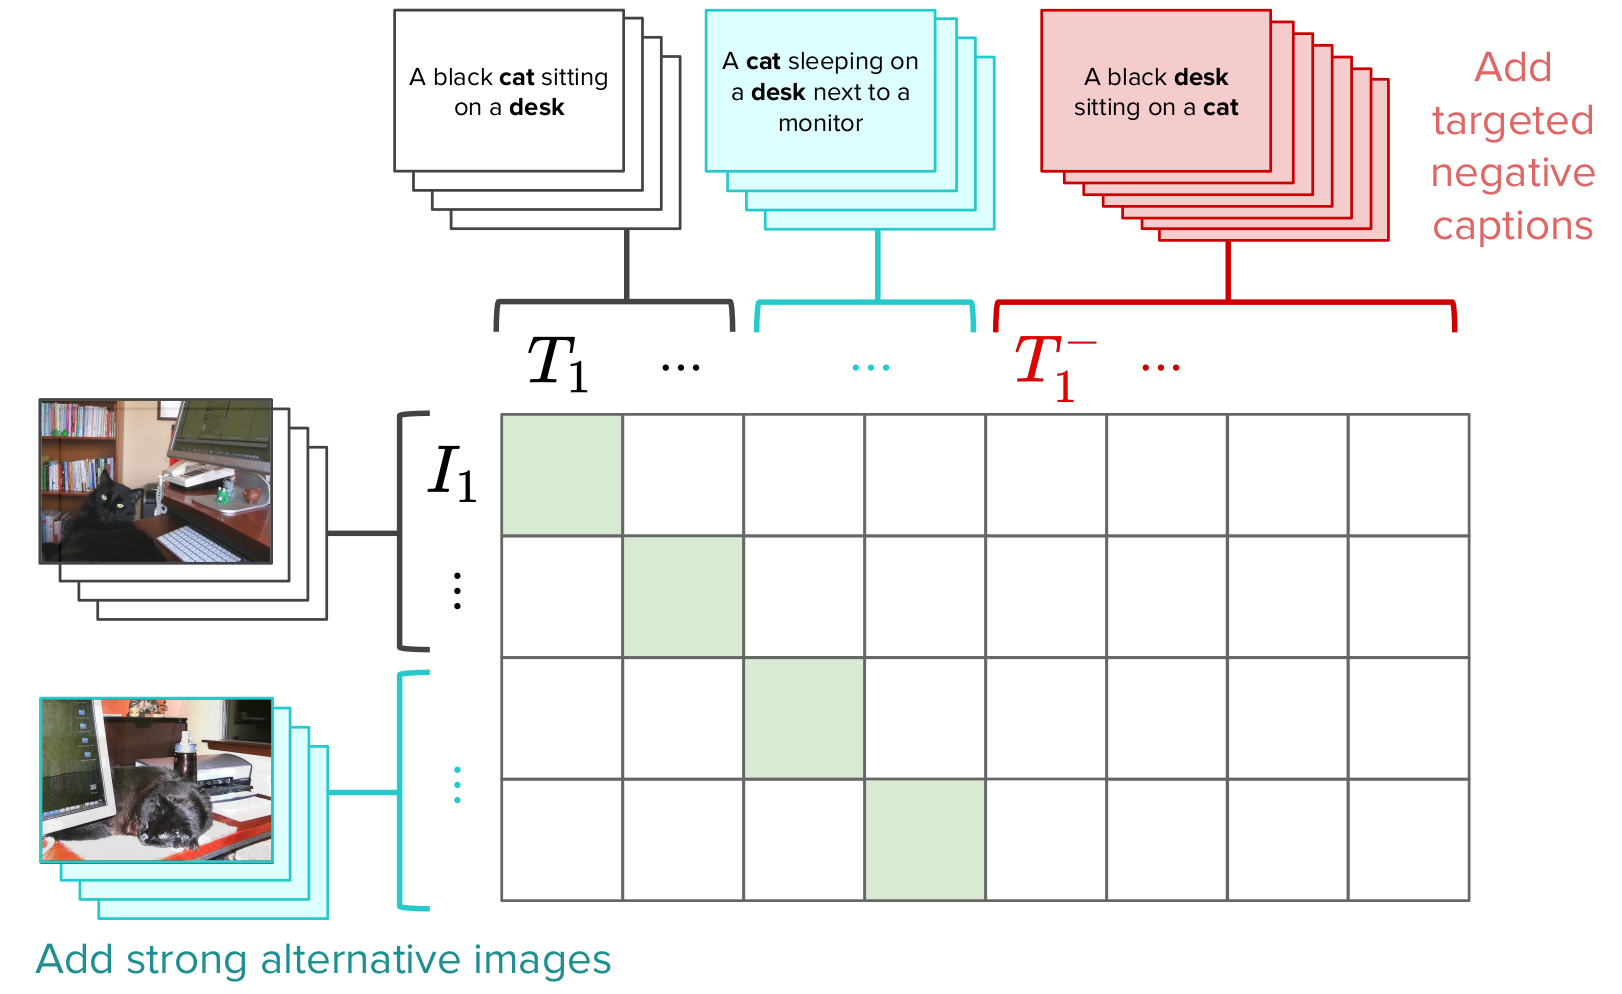
\includegraphics[width=0.8\textwidth]{bow_hard_negs.png}
	\caption{Hard negatives for contrastive learning, with generated negative
	captions and retrieved alternative images. Captions are generated by
	swapping various linguistic features, while images are sampled from 
	k-nearest neighbours. From~\citet{yuksekgonul2023when}.}
	\label{fig:bow_hard_negs}
\end{figure}


\section{Understanding in Video Language Models}
\label{sec:understandvidlm}

Here we discuss two papers that look at improving understanding in
\acrfullpl{vidlm} by extending the contrastive objectives with hard negatives
for verb understanding~\citep{momeni2023verbs}, and in before/after
relations~\citep{bagad2023testoftime}. 

\subsection{Verbs in Action}
\label{ssec:verbs}
\citet{momeni2023verbs} look at \acrshortpl{vidlm} trained with a contrastive
loss function, and find similar issues with verb understanding to those
identified by~\citet{yuksekgonul2023when}. They propose to generate hard
negatives with modified verb phrases using pre-trained \acrfullpl{llm}, as well
as introducing an additional verb phrase alignment loss which contrastively
compare a verb phrase from the positive caption to other verb phrases in the
batch to provide an additional focus on verbs to the model
(see~\cref{fig:vfc}). As in~\citet{yuksekgonul2023when}, models trained with
targeted alternatives improve performance for datasets that require
understanding of the targeted domain in both zero-shot and finetuning setups. 

\begin{figure}[t]
	\centering
	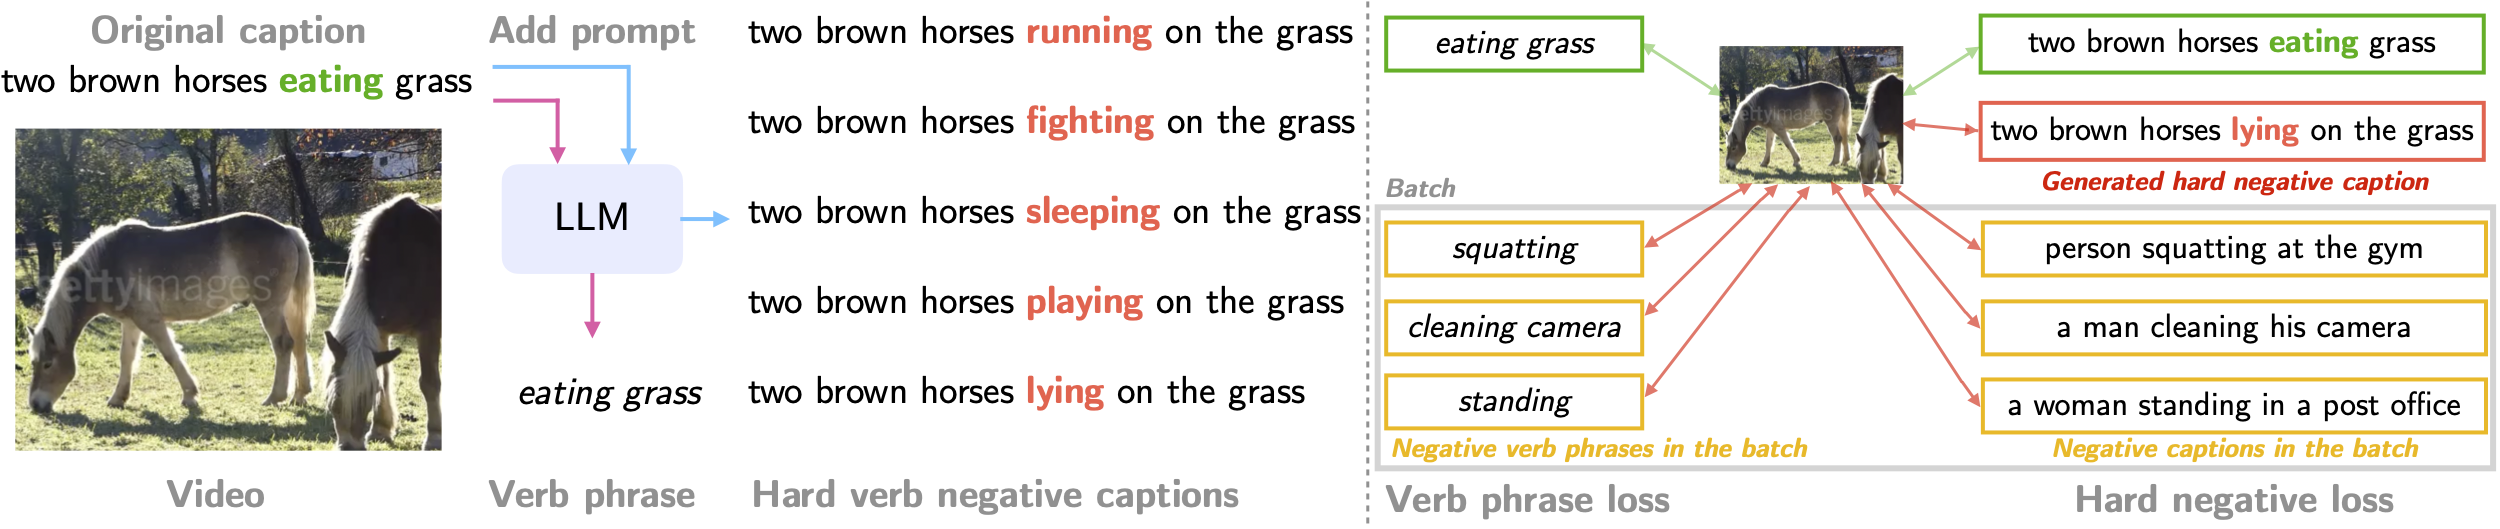
\includegraphics[width=\textwidth]{vfc.png}
	\caption{Verb-Focused Contrastive learning. Generated negative captions are
	added as hard negatives to the contrastive loss objective.
	From~\citet{momeni2023verbs}.}
	\label{fig:vfc}
\end{figure}


%InfoNCE loss, work in similar training styles for different domains
%\citep{momeni2023verbs, yuksekgonul2023when}.

\subsection{Test of Time}
\label{ssec:testoftime}
The most similar paper to our work is~\citet{bagad2023testoftime}. The authors
look at before/after relations in videos by using a synthetic dataset to
probe existing models. They construct videos containing pairs of events such
as ``a red circle appears before a yellow circle'', and create distractor
annotations by reversing the order of events but keeping the temporal relation
the same. On this time-order probing task, they find that existing models
perform no better than chance for the task of associating the correct
annotation to the video. They describe a post-pretraining strategy, Temporal
Adaptation by Consistency of Time-order (TACT), for improving the understanding
of before/after relations in \acrshortpl{vidlm}, where non-overlapping video
clips are stitched together and paired with a text description that consists of
the clip captions and a temporal relation, either before or after, to match the
order of the combined video clip (see~\cref{fig:tact}). A reversal function is
then applied to create hard negative examples by reversing the order of text
captions or video clips, which are included as negatives in the contrastive
post-pretraining objective.

\begin{figure}[t]
	\centering
	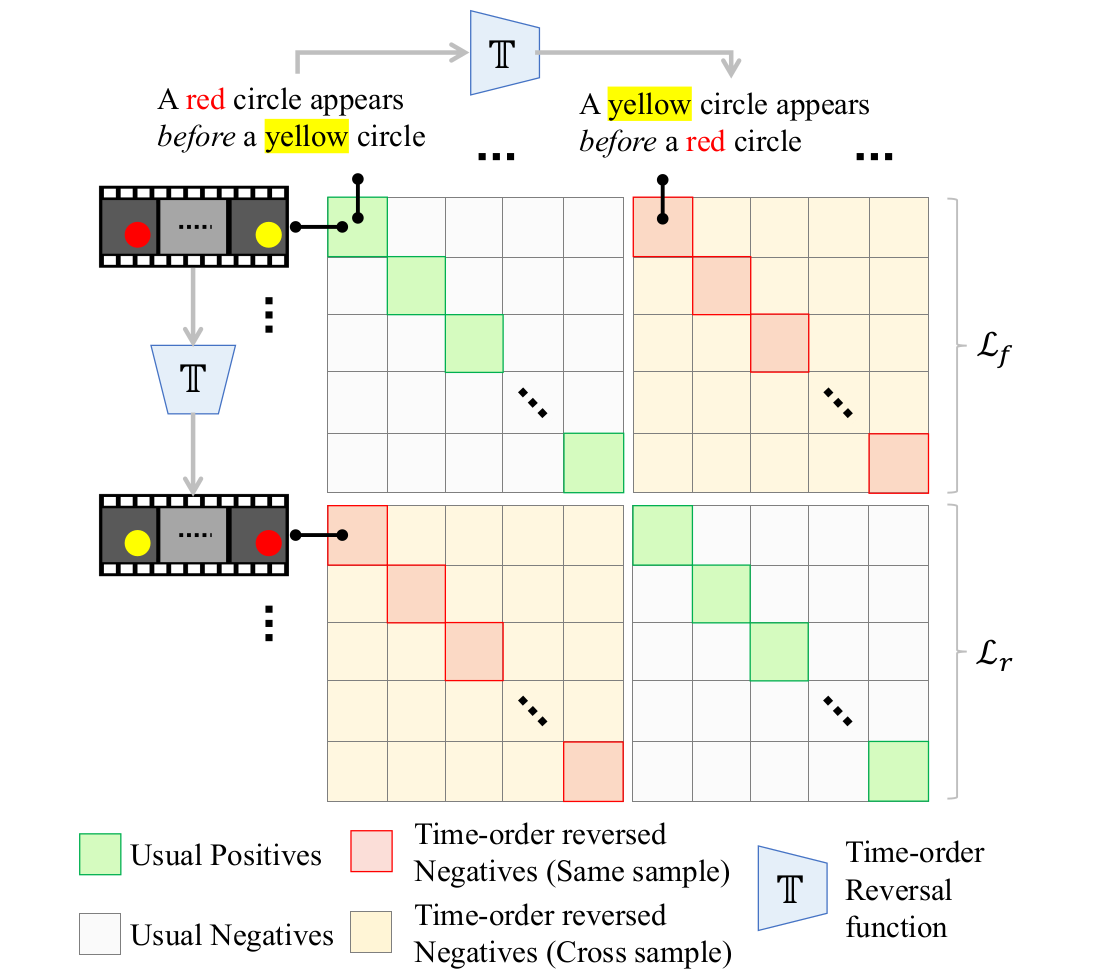
\includegraphics[width=0.8\textwidth]{tact.png}
	\caption{Temporal Adaptation by Consistency of Time-order. Extra negatives
	are included by reversing time-order in annotations and videos. Figure
	from~\citet{bagad2023testoftime}.}
	\label{fig:tact}
\end{figure}

They find that this approach improves performance on the time-order probing
task, with models much more likely to match the correct caption to the stitched
video clips. On downstream tasks, they find a mixed result. On video retrieval
tasks, on which they claim existing datasets have more of a bias towards
spatial understanding than temporal reasoning
(see~\cref{ssec:adaptvlm};~\citet{buch2022revisiting,lei2023revealing,luo2022clip4clip}),
the model performs slightly worse in general than without using the TACT
approach. On \acrlong{vidqa}, with temporally challenging datasets, there are
generally slight improvements. For example on the NExT-QA
ATP\textsubscript{hard} subset, the TACT model trained on clips from
TEMPO~\citep{hendricks2018tempo} achieves a zero-shot accuracy of 27.6,
compared to 25.0 on the baseline model.  However, on clips from the Charades
dataset~\citep{sigurdsson2016charades} the TACT performance is worse than the
Charades baseline model (25.2 vs 26.0). They find that the TACT model generally
improves performance on action recognition benchmark subsets which have been
identified as requiring temporal information. 

In comparison to~\citet{bagad2023testoftime}, we explore different ways of
probing temporal understanding, use a wider range of temporal relations with
full videos, and aim to gain a stronger relationship between frame and action
with the contrastive span objective. We provide a full comparison of our
approaches and results in~\cref{sec:tactcompare}. We now go on to describe the
datasets and models that we use in our approach.
